\chapter{Data Analysis}

    This section presents an analysis of data collected by \textsc{ATLAS} from $pp$ collisions at $\sqrt{s} = 13~\mathrm{TeV}$ in 2016, corresponding to datasets in Table \ref{tab:data_sim_samples}. The analysis focuses solely on the lepton+jets channel: one charged lepton, one neutrino, and four or more jets, two of which are $b$-tagged.


    \section{Event selection}
To select events corresponding to the lepton+jets channel, the dataset was filtered according to the criteria listed in Table~\ref{tab:cut}. These criteria aim to suppress Standard Model backgrounds to increase the chance of observing the \( t\bar{t} \) signal in the lepton+jets channel.


\begin{table}[h!]
\centering
\caption{Event Selection Criteria for the Lepton+Jets Channel}
\begin{tabular}{@{}lp{7cm}@{}}
\toprule
\textbf{Criteria} & \textbf{Requirement} \\ \midrule
Number of leptons & Exactly 1 (single-lepton channel) \\
Lepton \(p_T\) & \(> 50\) GeV  \\
Lepton \(|\eta|\) & \(< 2.5\) (detector acceptance) \\
Jet \(p_T\) & At least one jet with \(p_T > 80\) GeV \\
Number of jets & 3 -- 5 jets (targeting 4-jet \(t\bar{t}\) events) \\
b-tagging & At least one jet with MV2c10 \(> 0.83\) \\
Missing Energy $E_{\mathrm{T}}$ & $> 0$ \\
\bottomrule
\end{tabular}
\label{tab:cut}
\end{table}

% from \textbf{ ttbar\_example.root}, 
After applying event selection, Table~\ref{tab:efficiency_sidebyside} shows the overall efficiency across different datasets. The efficiency trend for all different Zprime masses indicates that the selection criteria are optimized for intermediate mass ranges around 2500-3000~GeV, with both lower and higher mass samples showing reduced selection efficiency.
\\

\begin{table}[htbp]
\centering
\caption{Overall Efficiency Across Datasets}
\label{tab:efficiency_sidebyside}
\begin{tabular}{@{}lc@{\hspace{2em}}lc@{}}
\toprule
\textbf{Dataset} & \textbf{Efficiency (\%)} & \textbf{Dataset} & \textbf{Efficiency (\%)} \\
\midrule
Data & 0.78 & Zprime1750 & 22.34 \\
diboson & 0.91 & Zprime2000 & 23.12 \\
single\_Top & 3.56 & Zprime2250 & 23.89 \\
ttbar & 6.15 & Zprime2500 & 24.73 \\
Zprime1000 & 16.17 & Zprime2750 & 26.45 \\
Zprime1250 & 19.02 & Zprime3000 & 25.18 \\
Zprime1500 & 20.67 & Zprime4000 & 2.83 \\
\bottomrule
\end{tabular}
\end{table}
\\

Moreover, Figure~\ref{fig:plot_event} presents examples of kinematic quantities illustrating low-level observables for the SM \(t\bar{t}\) background and a \(Z'\) signal with \(m_{Z'} = 1000\)~GeV. Figures~\ref{fig:plot_event} (a) and (b) show the jet \(p_T\) distributions for the background of SM \(t\bar{t}\) and the signal \(Z'\), respectively. In both cases, the jet \(p_T\) values are mostly below 600~GeV. Similarly, the lepton energy distributions \(lep_E\) shown in Figures~\ref{fig:plot_event} (c) and (d) are mostly below 1000 GeV. It is clear that the values in both plots overlap which means the cut based on this observable will not work well as it suppresses both the Standard Model background and the signal. This also occurs with other low-level observables such as missing transverse energy.



\begin{figure}[H]
    \centering
    % First row
    \begin{subfigure}[b]{0.48\textwidth}
        \centering
        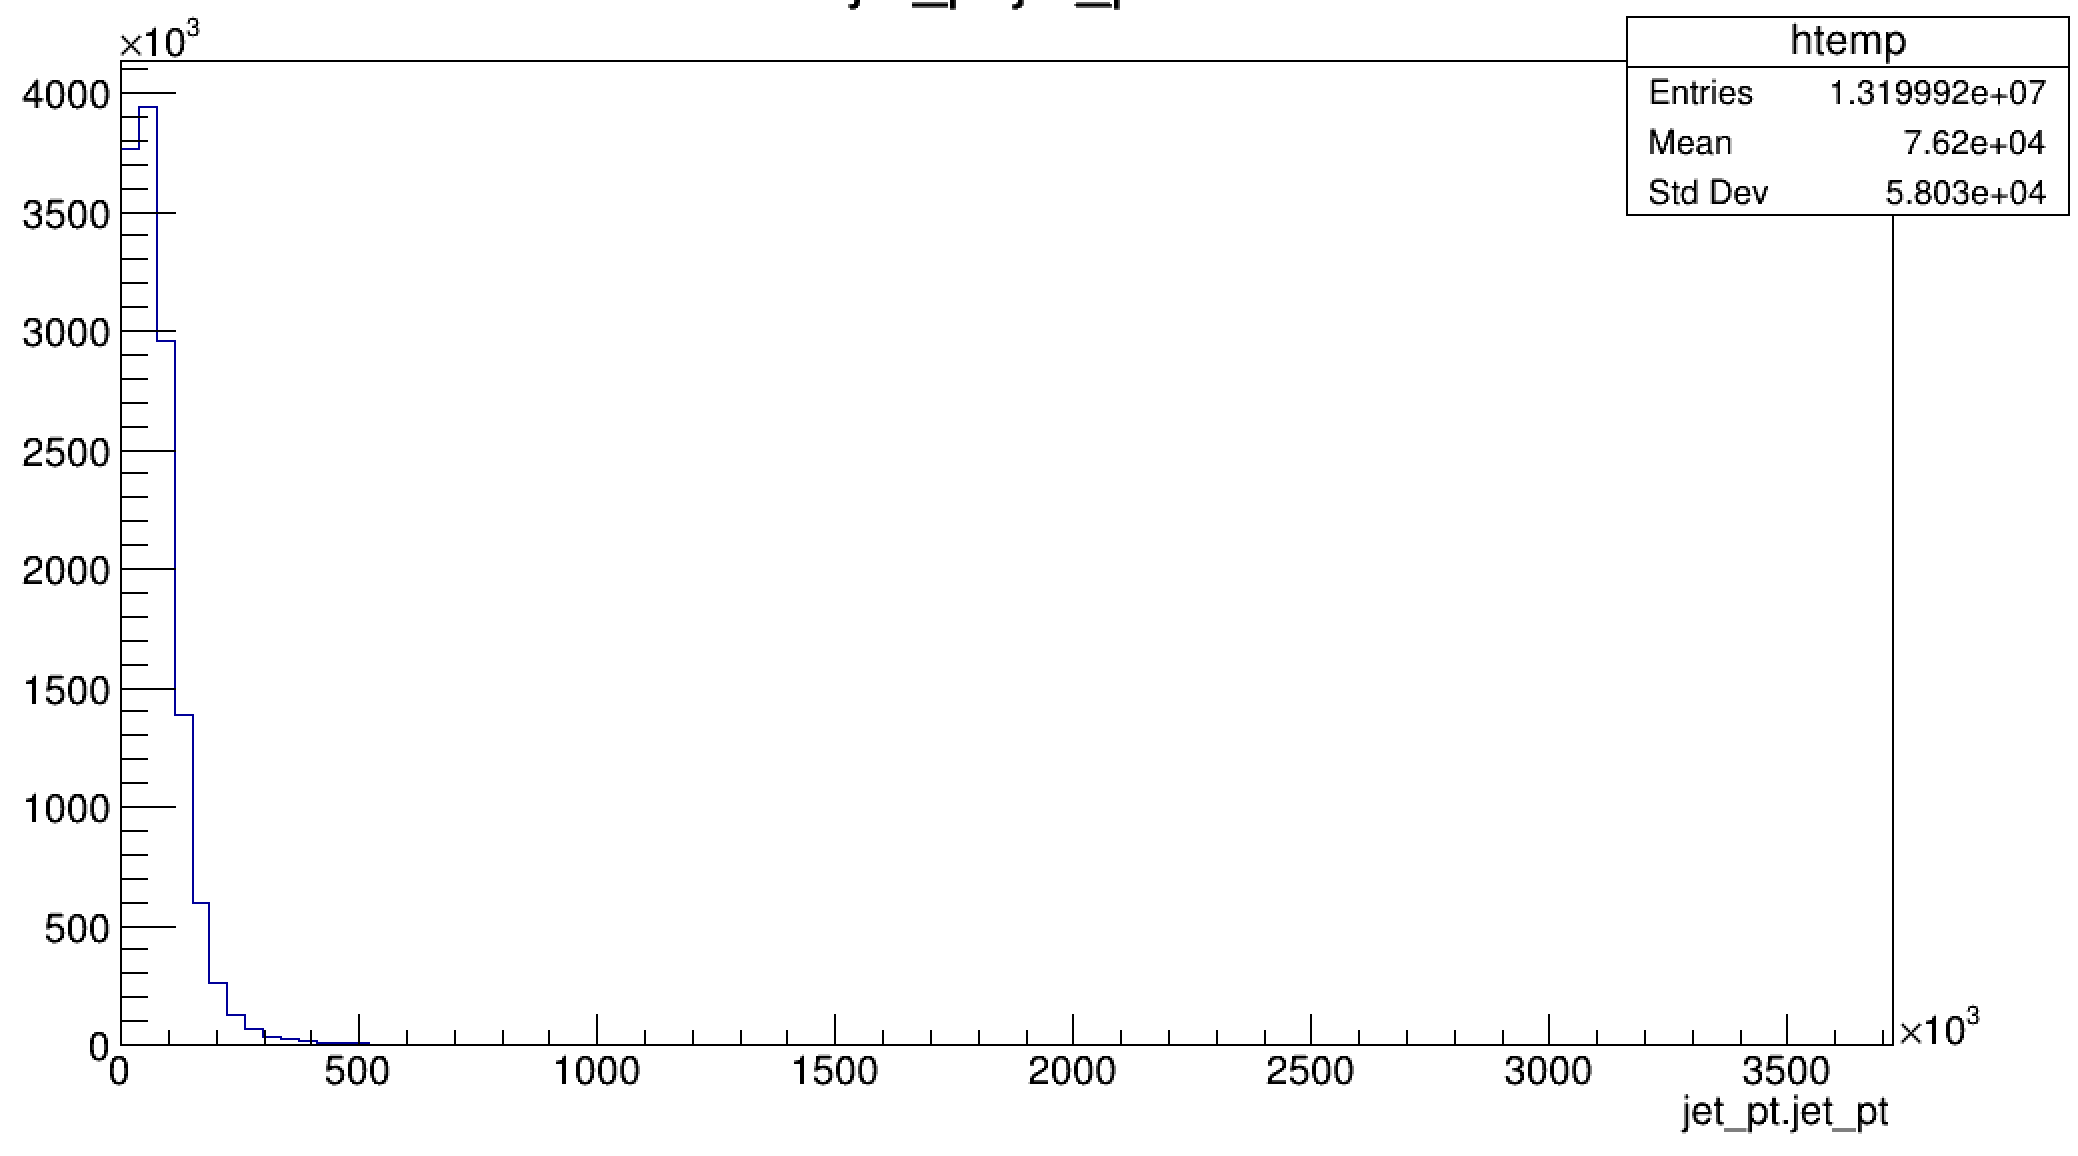
\includegraphics[width=0.8\textwidth]{Figure/low_jet_tt.png}
        \caption{Jet \(p_T\) distribution for the SM \(t\bar{t}\) background}
        \label{fig:bplus_mass_1}
    \end{subfigure}
    \hfill
    \begin{subfigure}[b]{0.48\textwidth}
        \centering
        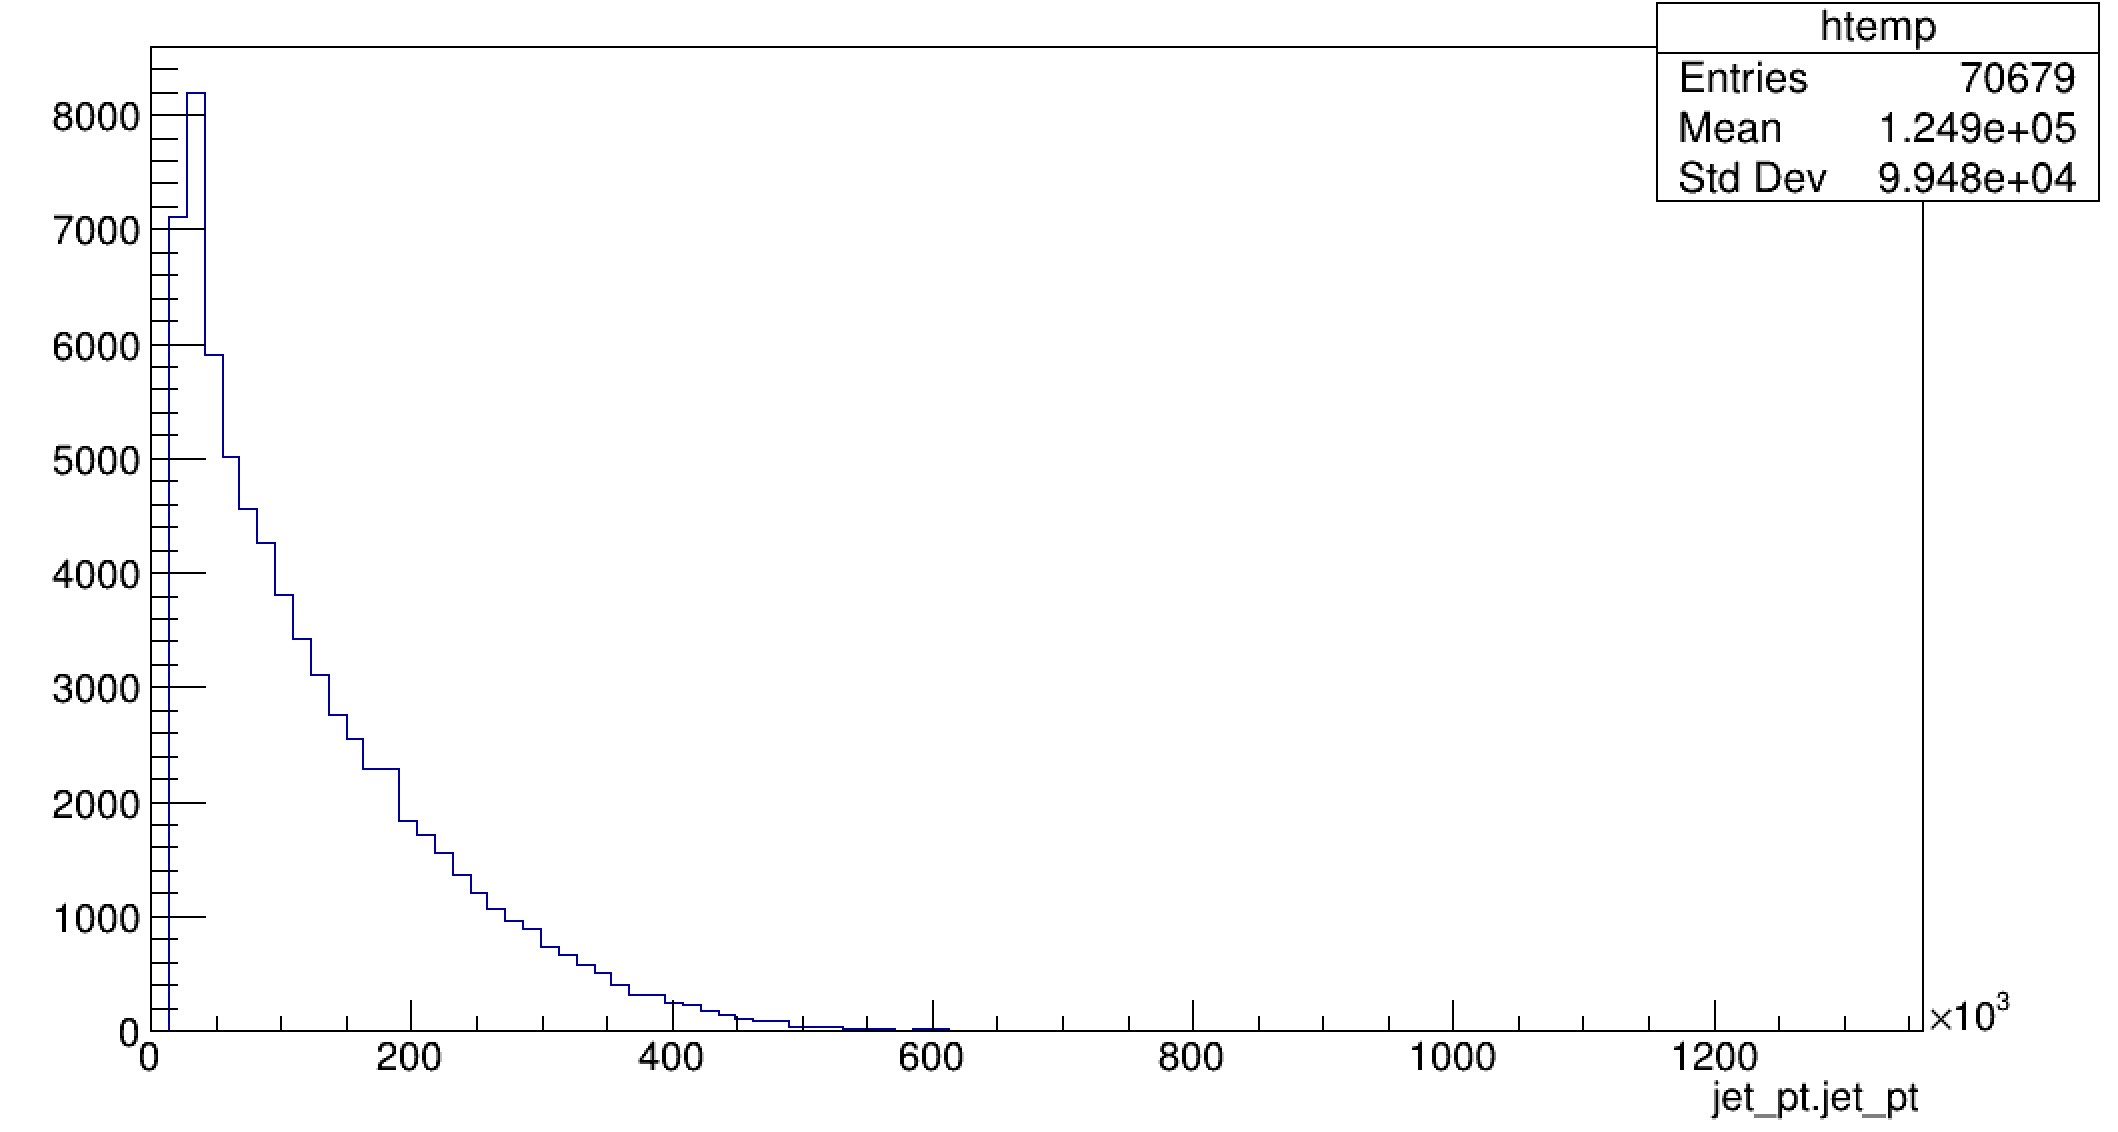
\includegraphics[width=0.8\textwidth]{Figure/low_jet_Z.png}
        \caption{Jet \(p_T\) distribution for the \(Z'\) signal}
        \label{fig:bminus_mass_1}
    \end{subfigure}

    \vspace{0.5cm} % Space between rows

    % Second row
    \begin{subfigure}[b]{0.48\textwidth}
        \centering
        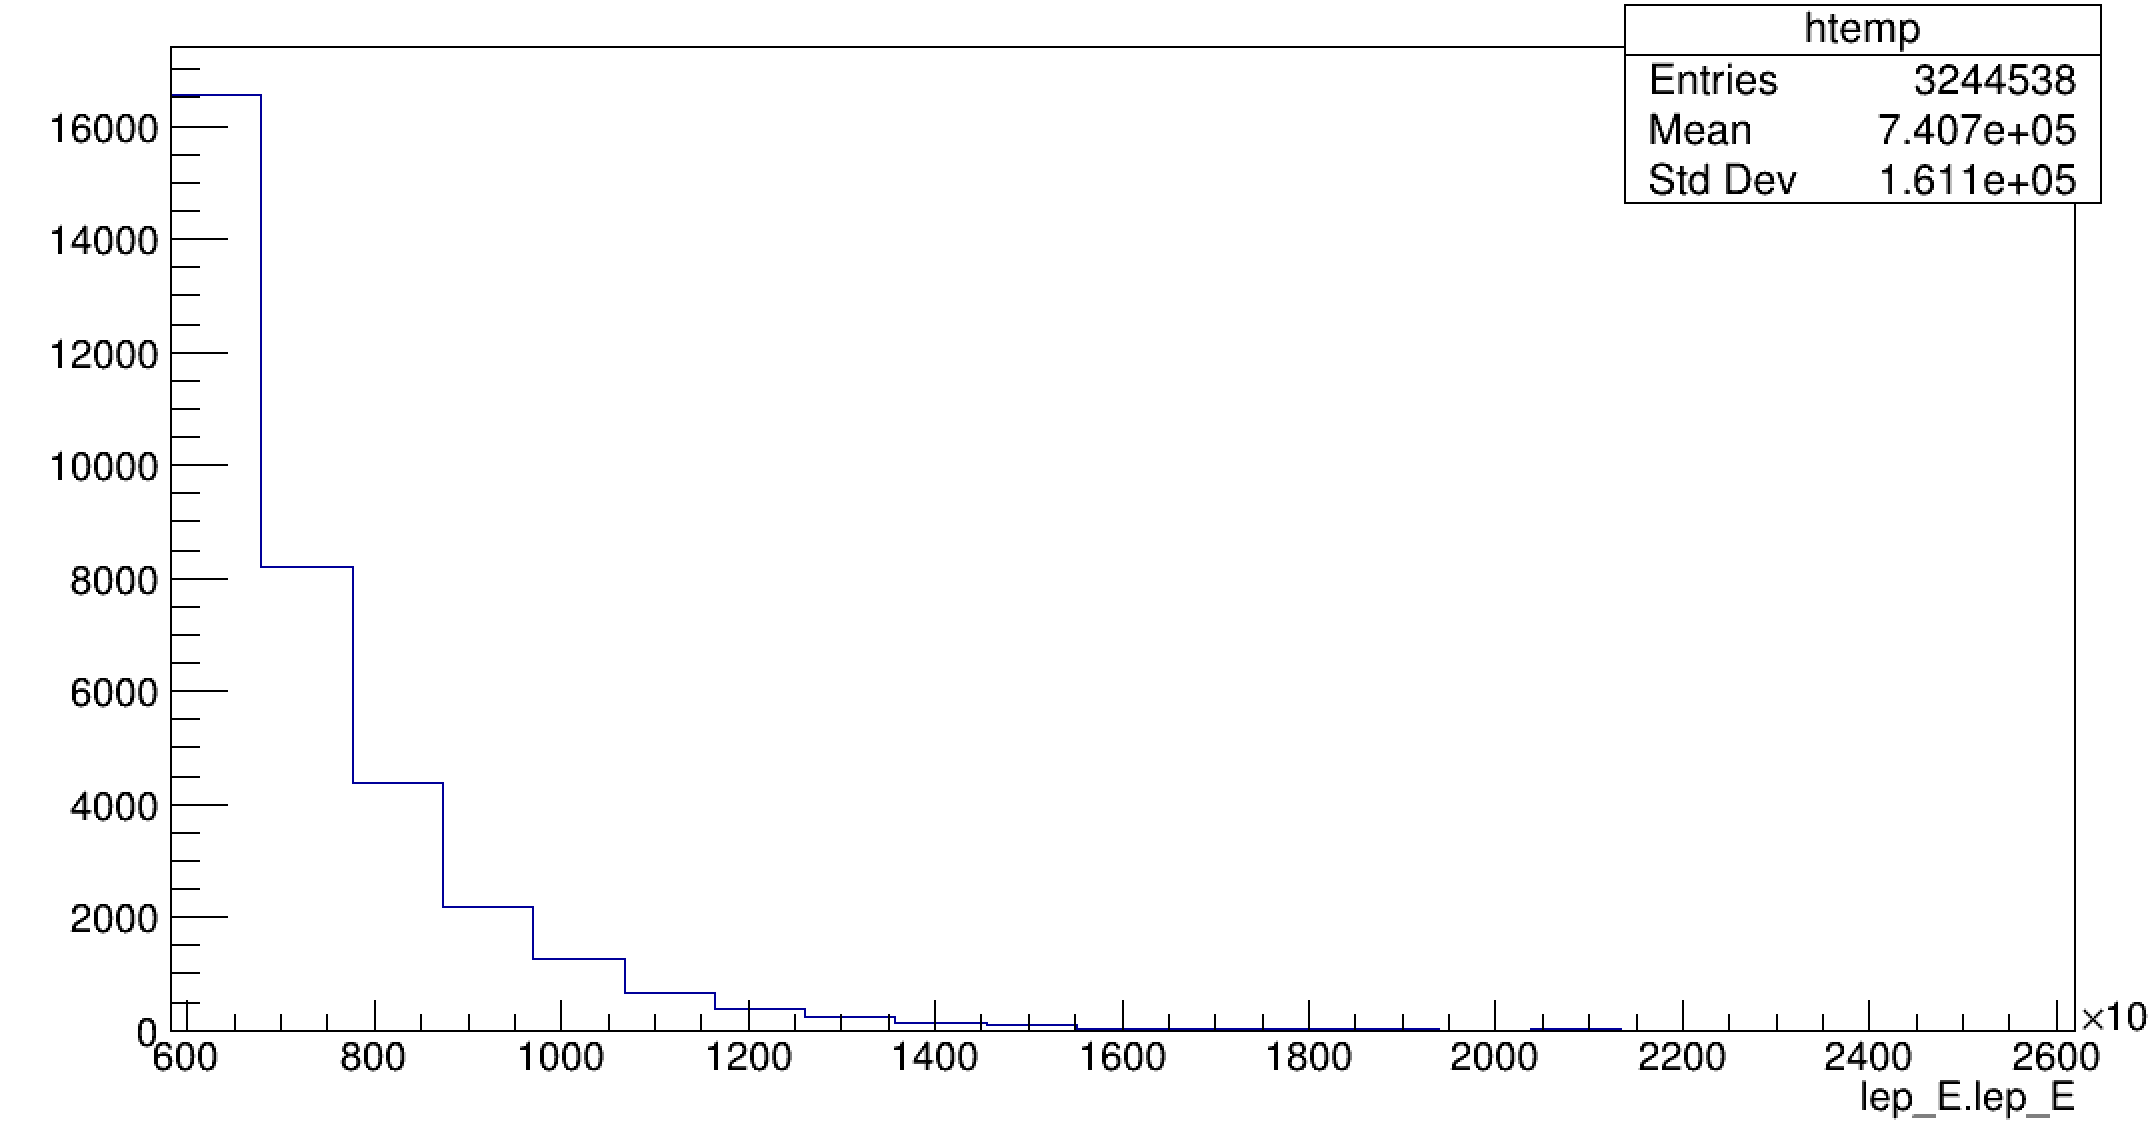
\includegraphics[width=0.8\textwidth]{Figure/low_elep_tt.png}
        \caption{Lepton energy distribution \(lep_E\) for the SM \(t\bar{t}\) background}
        \label{fig:bplus_mass_2}
    \end{subfigure}
    \hfill
    \begin{subfigure}[b]{0.48\textwidth}
        \centering
        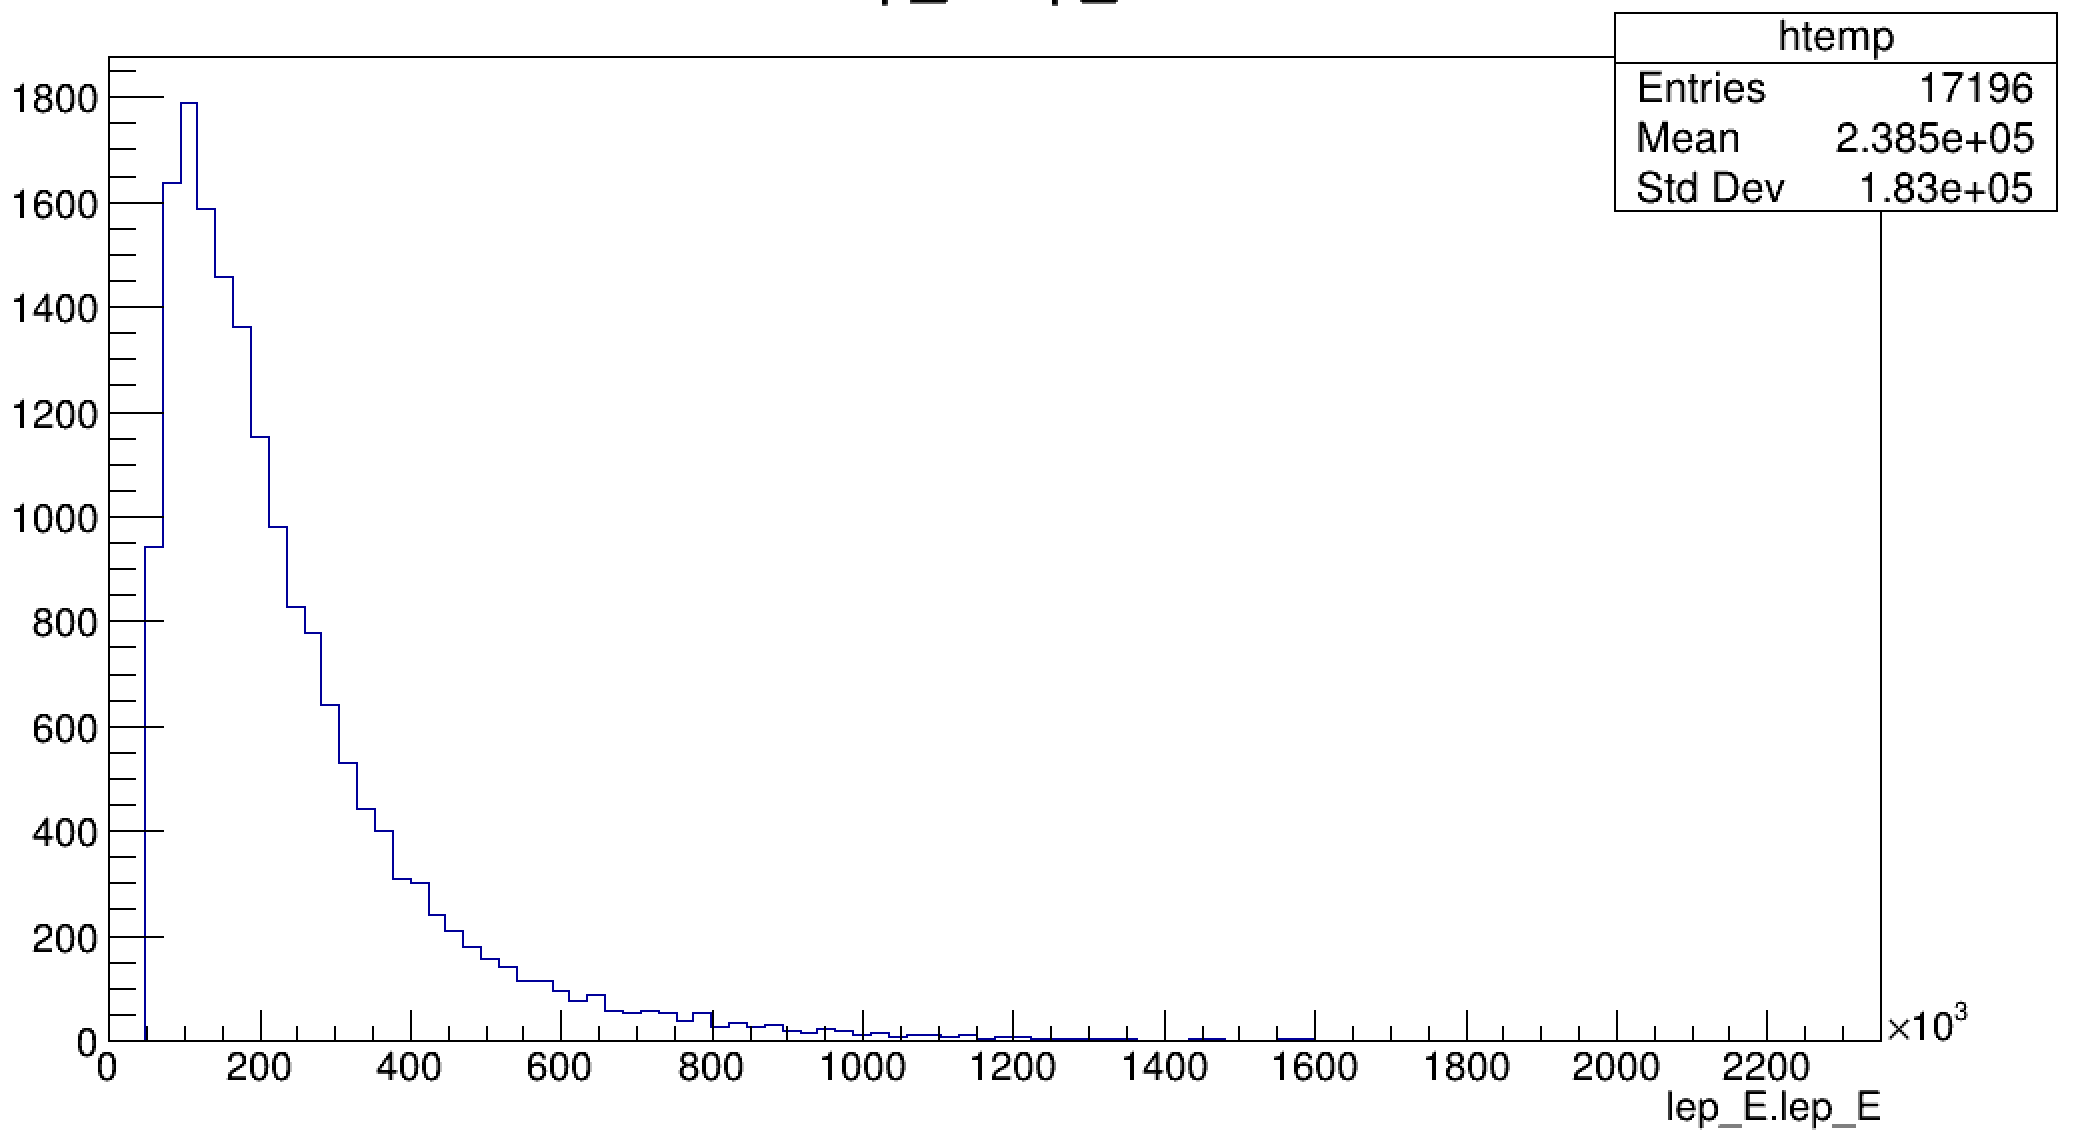
\includegraphics[width=0.8\textwidth]{Figure/low_elep_Z.png}
        \caption{Lepton energy distribution \(lep_E\) for the \(Z'\) signal}
        \label{fig:bminus_mass_2}
    \end{subfigure}

    \caption{
    Distributions of kinematic variables after event selection. (a) and (b) show jet transverse momentum (\(p_T\)) for the SM \(t\bar{t}\) background and \(Z'\) signal, respectively. (c) and (d) show lepton energy \(lep_E\) distributions for the SM \(t\bar{t}\) background and \(Z'\) signal, respectively}
    \label{fig:plot_event}
\end{figure}



    The discriminating power of the low-level observables is insufficient for further analysis. Therefore, high-level observables are introduced to improve the separation between signal and background. High-level observables use combined information from low-level observables to better tell the signal apart from the background. This analysis identifies several suitable high-level variables, selected from the following:


\begin{itemize}
    \item \(E_{\text{T}}^{miss}\), the missing transverse momentum magnitude;
    \item Azimuthal angle difference between \(E_{\text{T}}^{miss}\) and the lepton;
    \item Invariant mass of the three highest-\(p_T\) jets;
    \item Invariant mass of the four highest-\(p_T\) jets, lepton, and neutrino.
    \item Pseudorapidity of the system of four highest-\(p_T\) jets, lepton, and neutrino.
\end{itemize}

    Through trial and error, the invariant masses of the three and four highest-\(p_T\) jets, lepton, and neutrino were selected as extra event selection criteria. Figure~\ref{fig:plot_high} shows a comparison between the SM \(t\bar{t}\) background and the \(Z'\) signal with \(m = 1000\)~GeV. The three highest-\(p_T\) jets in panels (a) and (b) exhibit strong discriminative power: for the SM \(t\bar{t}\), the distribution peaks near 100~GeV, while the \(Z'\) signal shows a Gaussian-like peak around 500~GeV. Similarly, the four highest-\(p_T\) jets, neutrino and lepton in panels (c) and (d) display a clear skew in opposite directions between the two samples.



\begin{figure}[H]
    \centering
    % First row
    \begin{subfigure}[b]{0.48\textwidth}
        \centering
        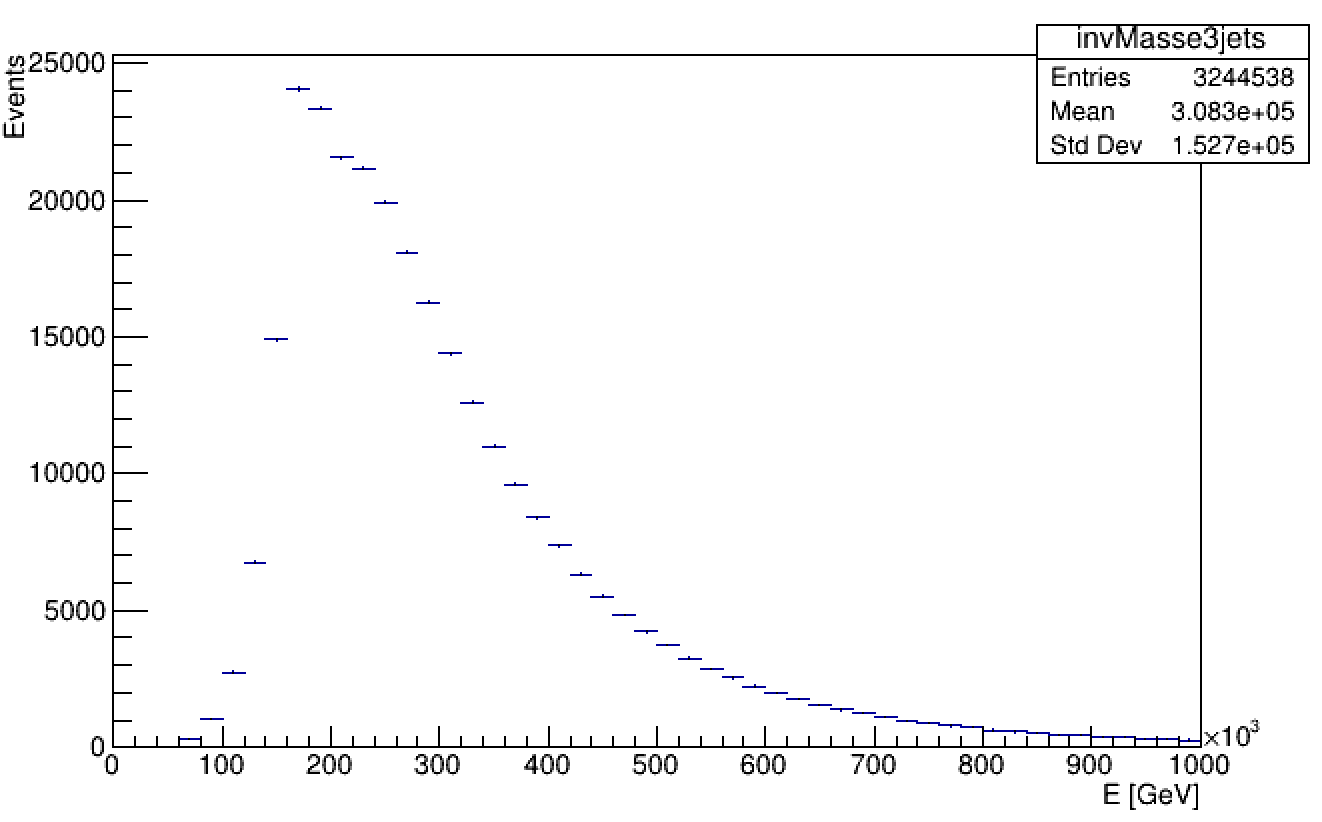
\includegraphics[width=0.8\textwidth]{Figure/high_3jet_tt.png}
        \caption{Jet \(p_T\) distribution for the three highest-\(p_T\) jets, lepton, and neutrino in the SM \(t\bar{t}\) background}
        \label{fig:plot_high_a}
    \end{subfigure}
    \hfill
    \begin{subfigure}[b]{0.48\textwidth}
        \centering
        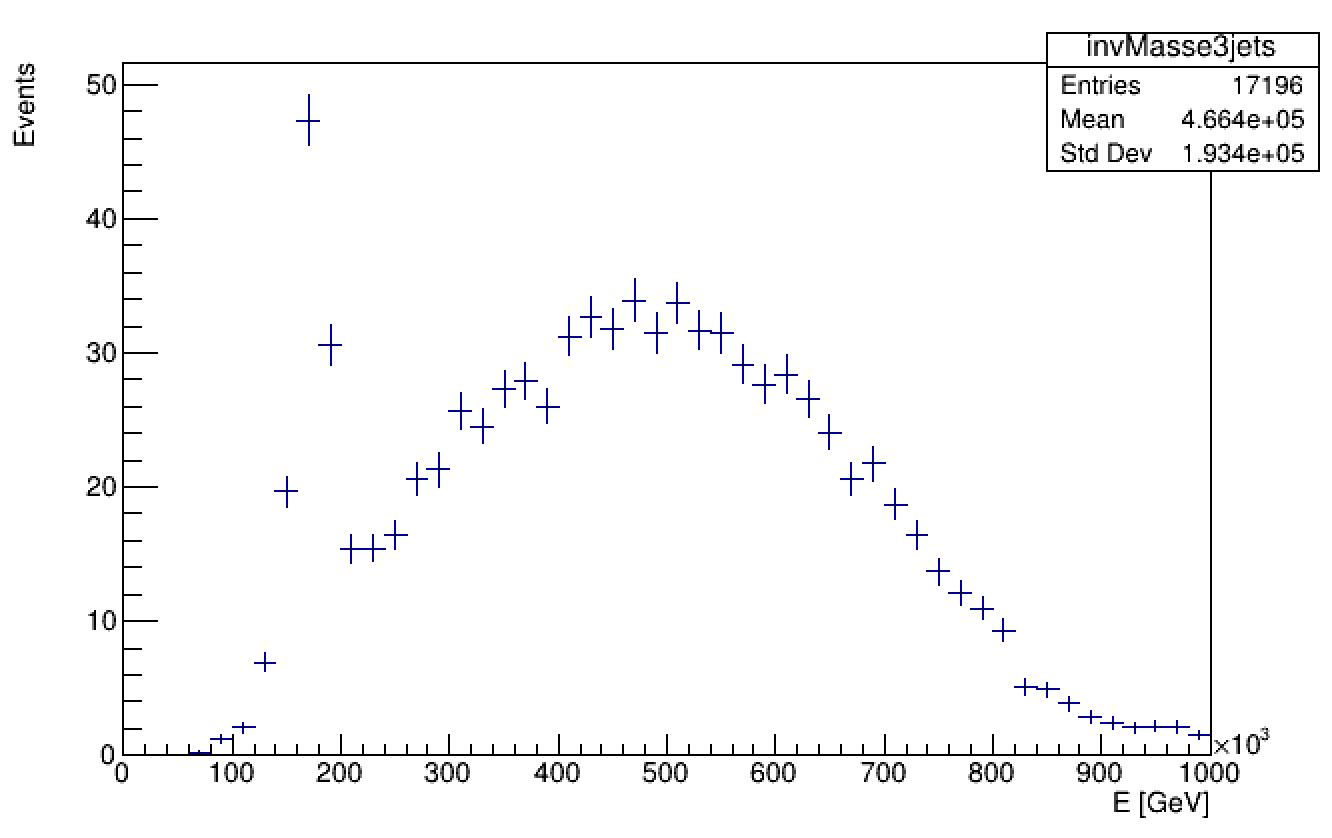
\includegraphics[width=0.8\textwidth]{Figure/high_3jet_zz.png}
        \caption{Jet \(p_T\) distribution for the three highest-\(p_T\) jets in the \(Z'\) signal}
        \label{fig:plot_high_b}
    \end{subfigure}

    \vspace{0.5cm} % Space between rows

    % Second row
    \begin{subfigure}[b]{0.48\textwidth}
        \centering
        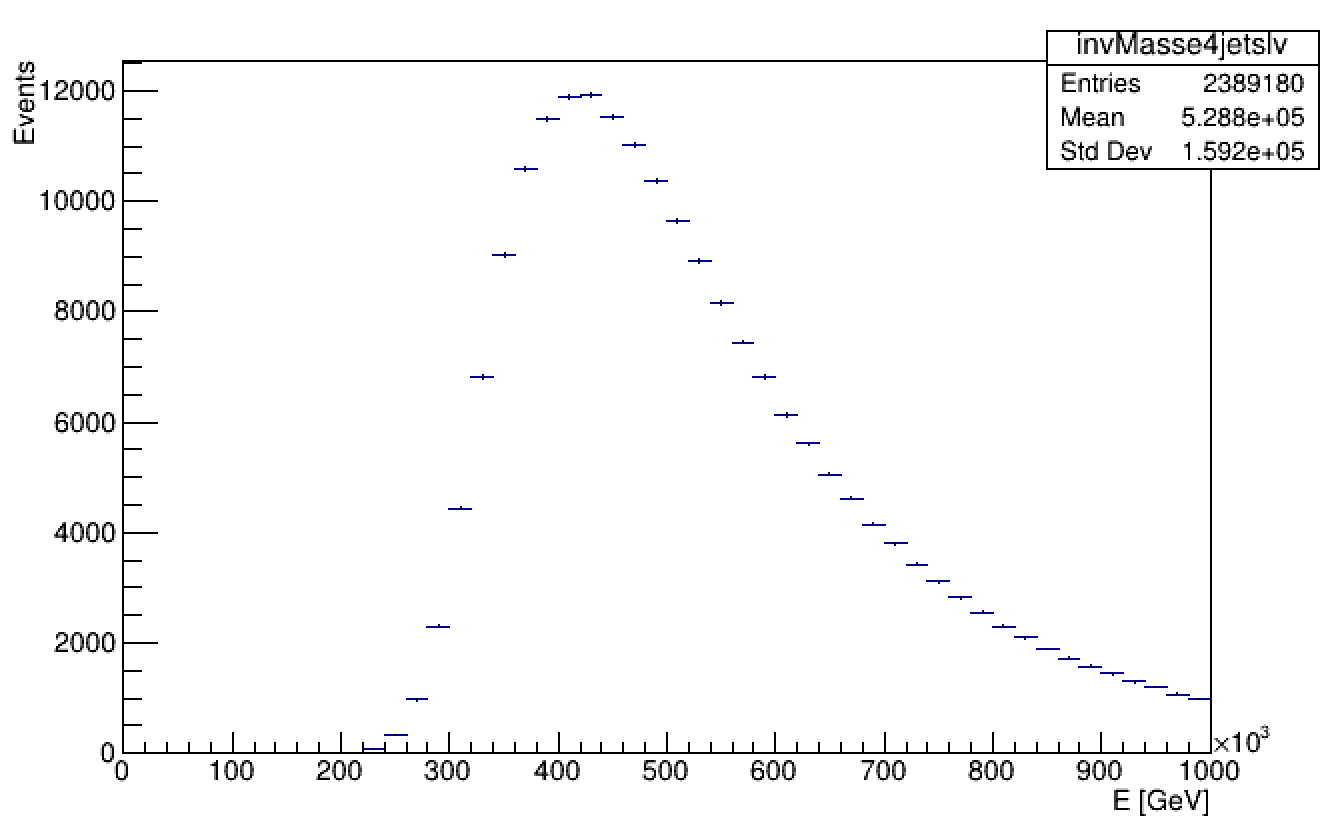
\includegraphics[width=0.8\textwidth]{Figure/high_4jet_tt.png}
        \caption{Jet \(p_T\) distribution for the 4th highest-\(p_T\), lepton, and neutrino jet in the SM \(t\bar{t}\) background}
        \label{fig:plot_high_c}
    \end{subfigure}
    \hfill
    \begin{subfigure}[b]{0.48\textwidth}
        \centering
        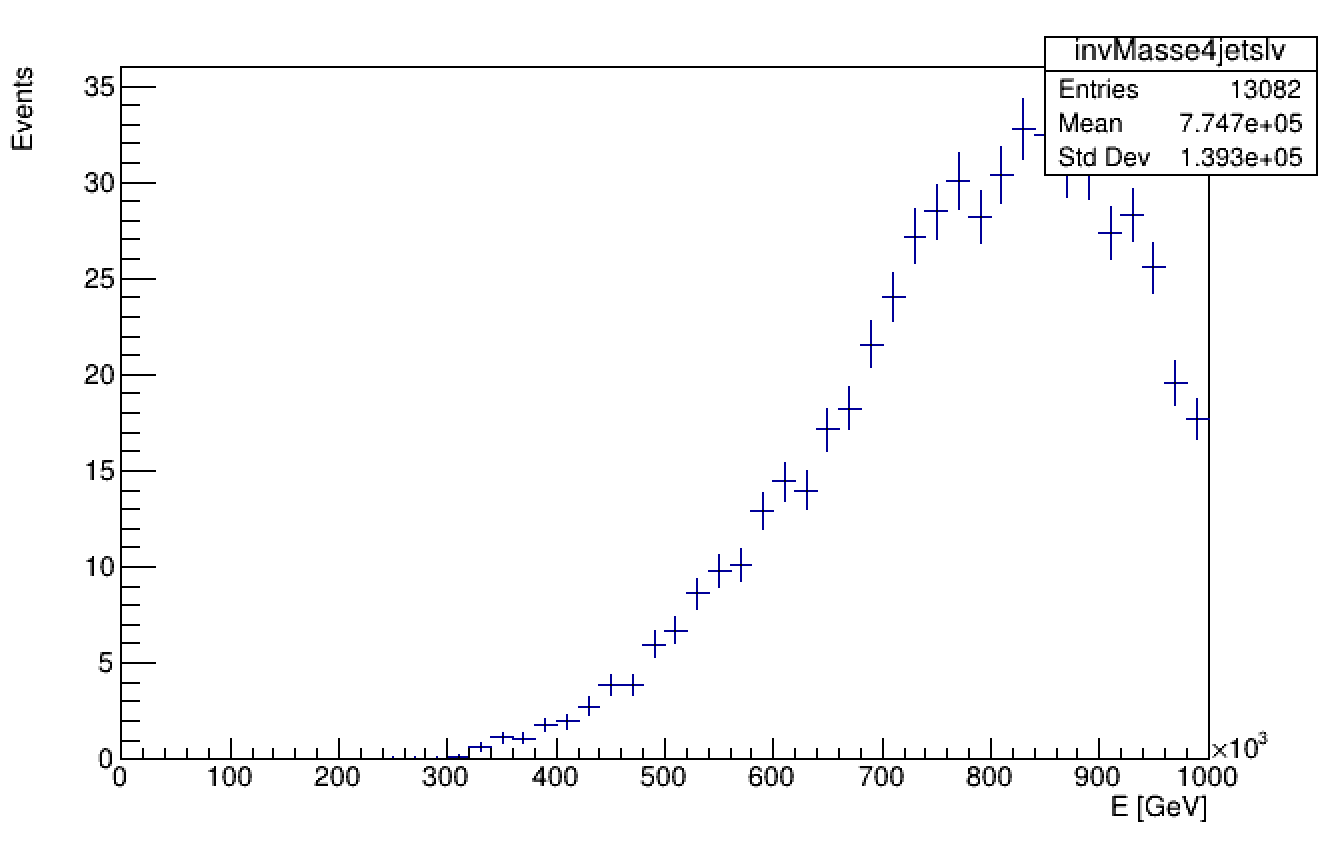
\includegraphics[width=0.8\textwidth]{Figure/high_4jet_zz.png}
        \caption{Jet \(p_T\) distribution for the 4th highest-\(p_T\) jet in the \(Z'\) signal}
        \label{fig:plot_high_d}
    \end{subfigure}

    \caption{Comparison between the SM \(t\bar{t}\) background and the \(Z'\) signal with \(m = 1000\)~GeV.}
    \label{fig:plot_high}
\end{figure}
Until this point, the event selection using both low- and high-level observables filters the data expected to be used for next analysis.


%%Panels (a) and (b) show the jet \(p_T\) distributions for the three highest-\(p_T\) jets, where the SM \(t\bar{t}\) background peaks near 100~GeV while the \(Z'\) signal peaks around 500~GeV. Panels (c) and (d) show the jet \(p_T\) distributions of the 4th highest-\(p_T\) jet, lepton, and neutrino, exhibiting opposite skewness between the SM background and the signal.
    %%% Explaination




    




    \section{Agreement of Simulation and Data}
    
    The next step in the analysis is to ensure data–MC agreement so that any sign of new physics can be studied under the background-only hypothesis. First, considering that the expected number of events \( N_{\text{exp}} \) represents the number of events detected for a given process.

    \begin{equation}
     N_{\text{exp}} = \mathcal{L} \cdot \sigma \cdot \varepsilon \cdot A
    \label{eq:nexp}
    \end{equation}

    Where \(\mathcal{L}\) is the integrated luminosity, \(\sigma\) is the production cross-section of the process, \(\varepsilon\) is the selection efficiency, and \(A\) is the detector acceptance.
    \\
    
    To achieve the background-only hypothesis, all simulated events must be normalized to the integrated luminosity of the dataset. Each MC event is assigned a weight \( w \) which adjusts the contribution of that event so that the total sum of weighted events matches \( N_{\text{exp}} \):

    \begin{equation}
    w = \frac{w_{\text{MC}} \cdot \mathcal{L} \cdot \sigma}{\sum w_{\text{MC}}}
    \label{eq:weight}
    \end{equation}

Here, \( w_{\text{MC}} \) is the generator weight of the event and \(\sum w_{\text{MC}} \) is the sum of all generator weights before any selection is applied. This weighting ensures the MC sample is normalized to the expected number of events observed in the data. 
So far Monte Carlo event weights \( w \) scale individual events so their sum matches the expected total number of events \( N_{\text{exp}} \) ensuring the simulation correctly represents the interested process.
\\

Figure~\ref{fig:plot_stack} shows example distributions in a stacked plot comparing the agreement between simulation and data. It is evident that there are regions with significant uncertainties where the data do not align well with the simulation, suggesting that improvements in the underlying theory or simulation techniques may be necessary. Such effects are clearly observed in the \(p_T\) distributions of the lepton (a) and jets (b). However for high-level observables such as the four-\(p_T\) (d) jets, neutrino and lepton the simulation and data show good agreement. Hence, this level of agreement is sufficient to perform a statistical analysis for the search for a \(t\bar{t}\) resonance.
\\

\begin{figure}[H]
    \centering
    % First row
    \begin{subfigure}[b]{0.48\textwidth}
        \centering
        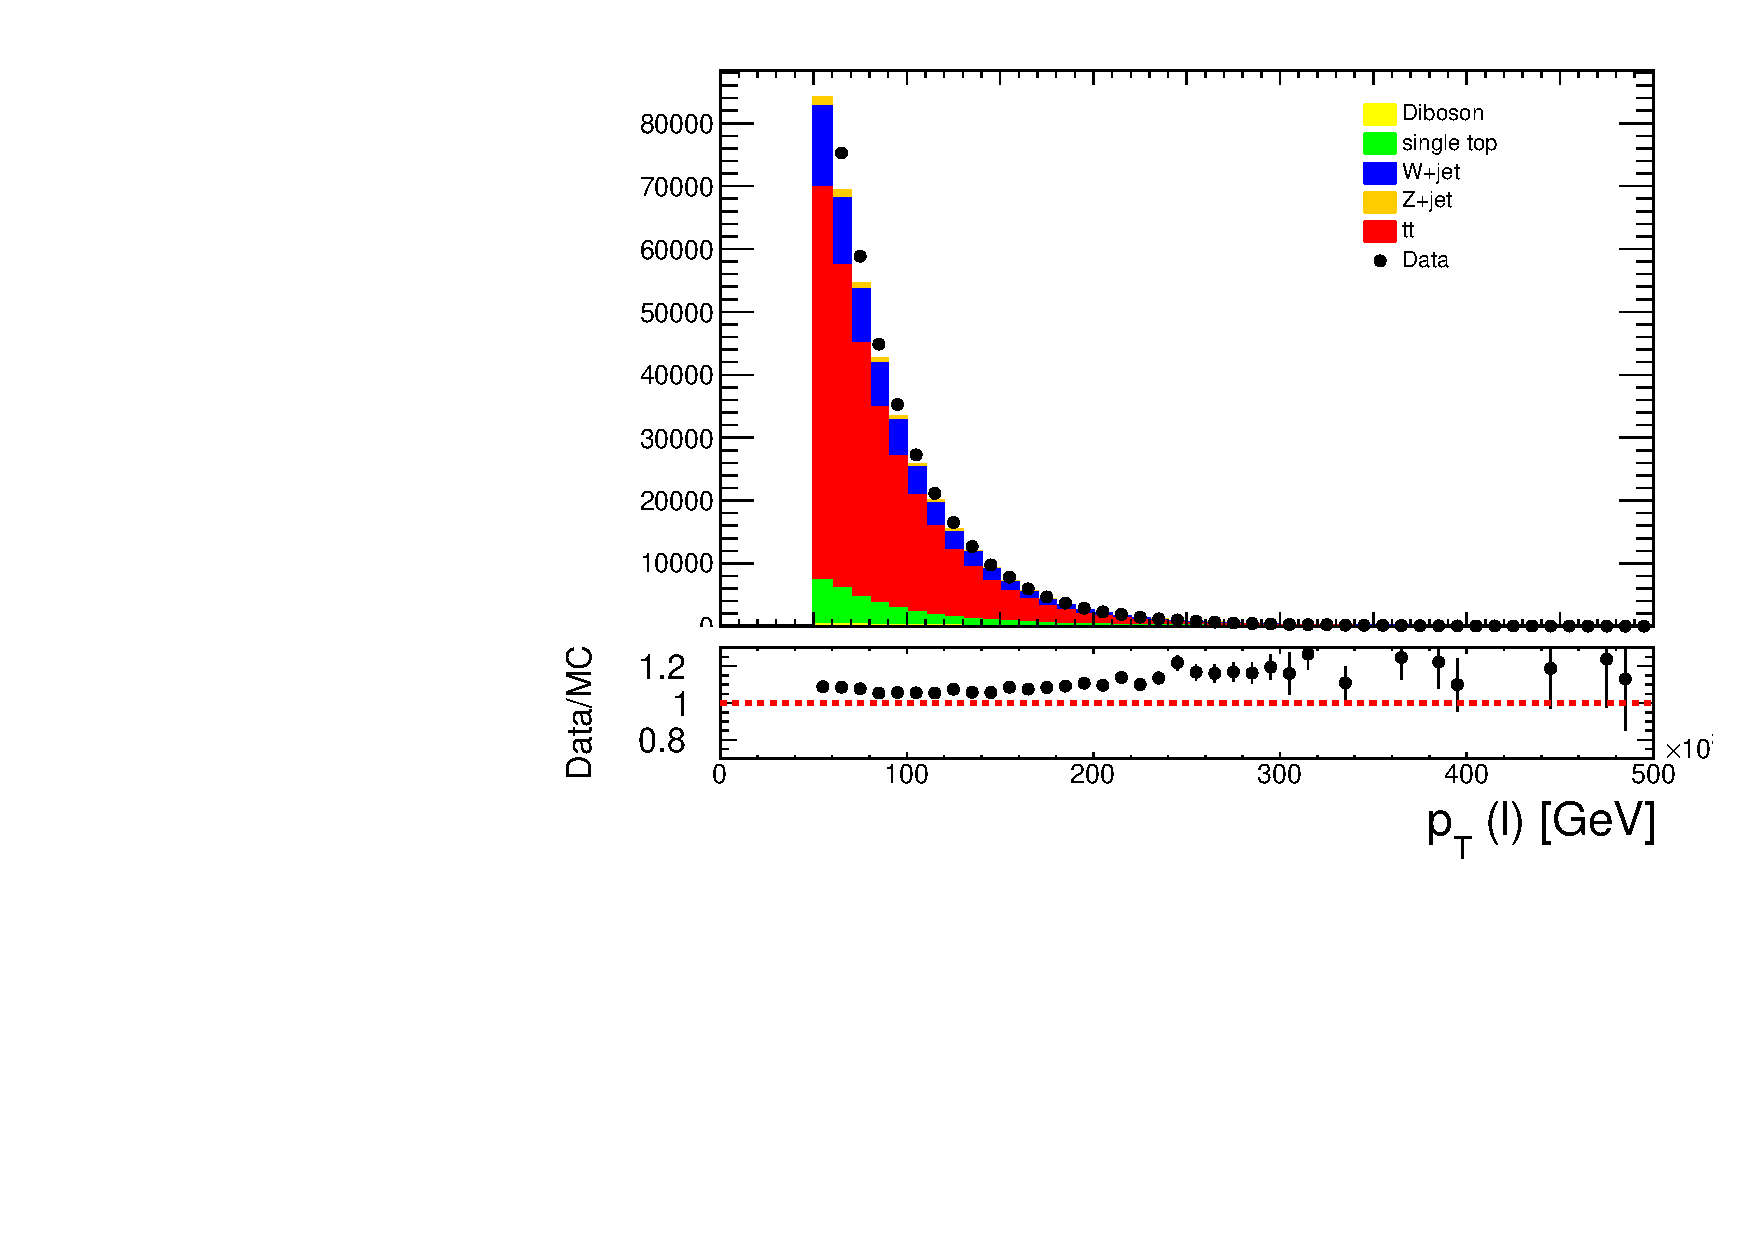
\includegraphics[width=\textwidth]{Figure/h_mc_lep_pt_stacked.pdf}
        \caption{Lepton \(p_T\) distribution}
        \label{fig:plot_high_a}
    \end{subfigure}
    \hfill
    \begin{subfigure}[b]{0.48\textwidth}
        \centering
        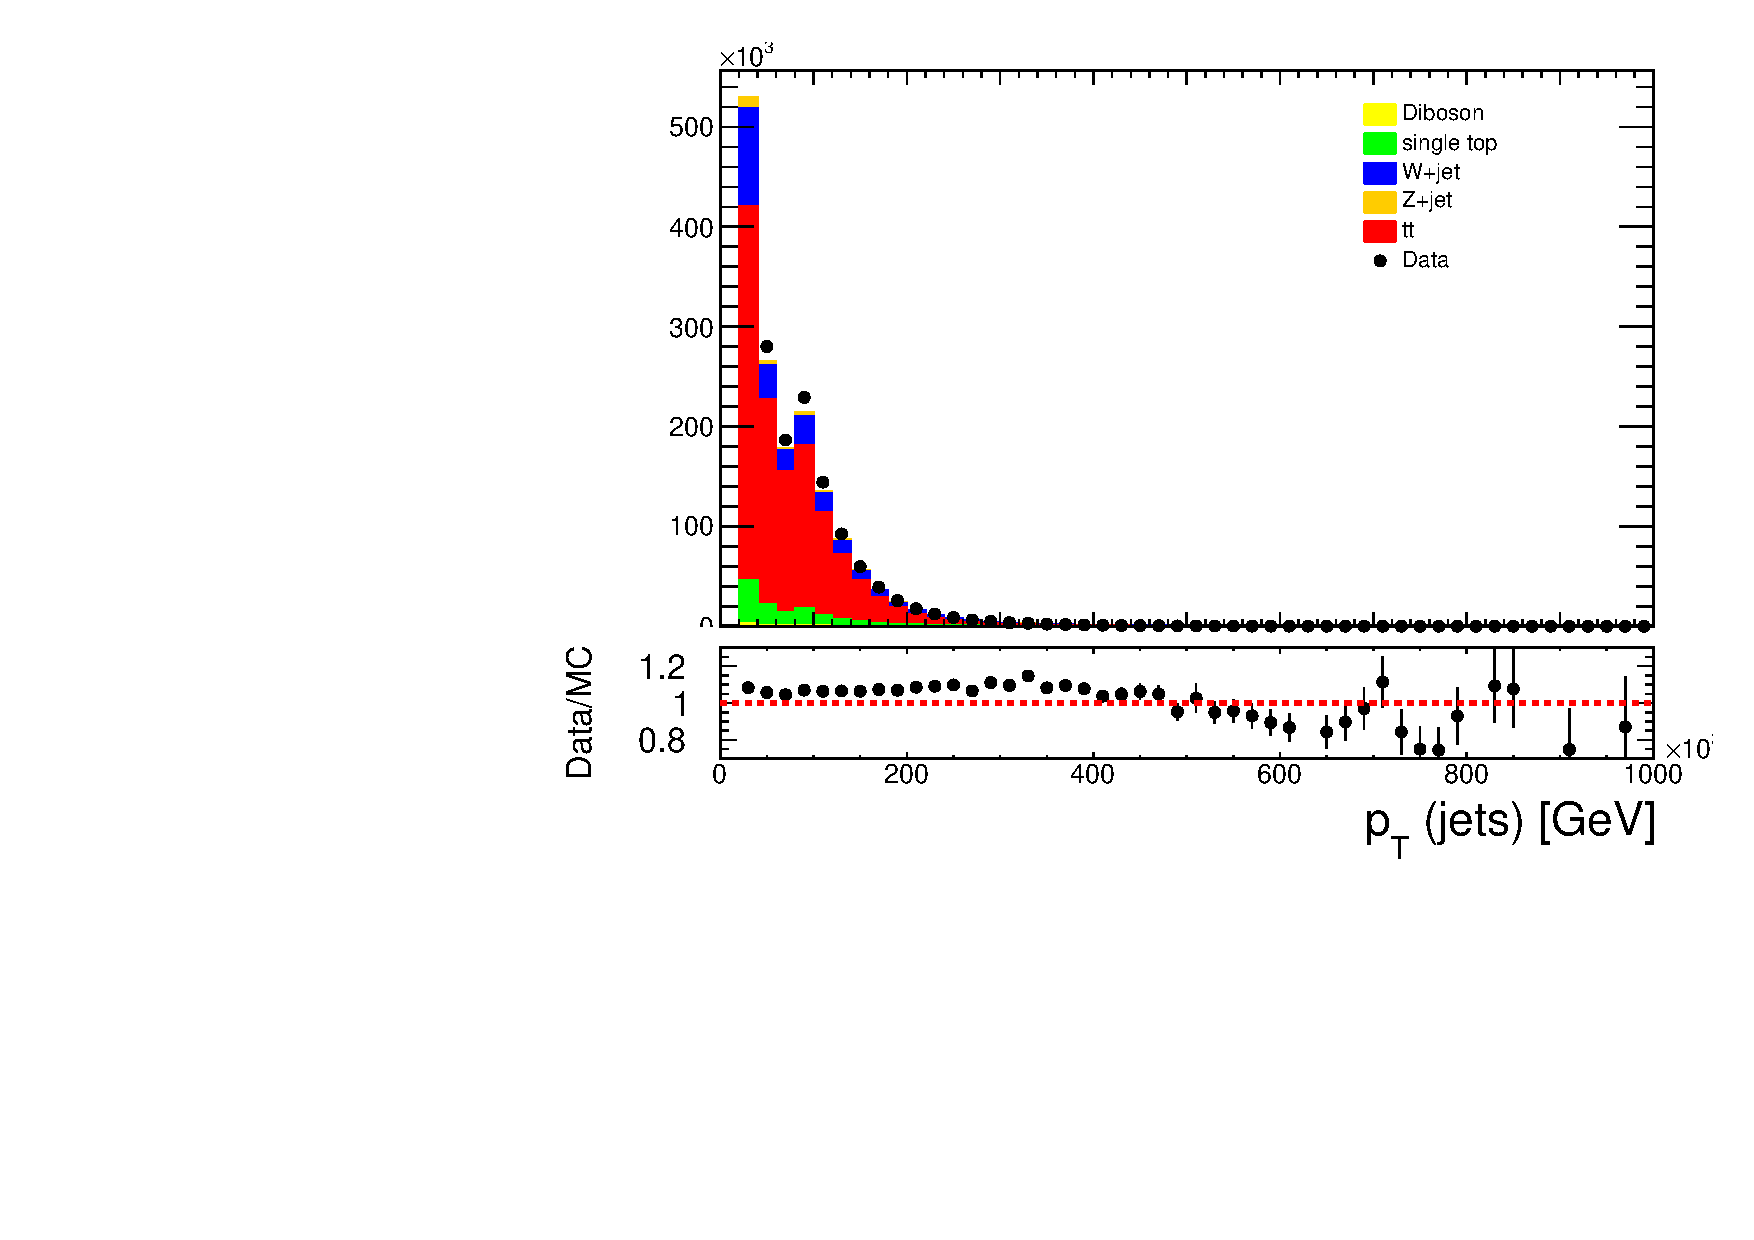
\includegraphics[width=\textwidth]{Figure/h_mc_jet_pt_stacked.pdf}
        \caption{Jet \(p_T\) distribution}
        \label{fig:plot_high_b}
    \end{subfigure}

    \vspace{0.5cm} % Space between rows

    % Second row
    \begin{subfigure}[b]{0.48\textwidth}
        \centering
        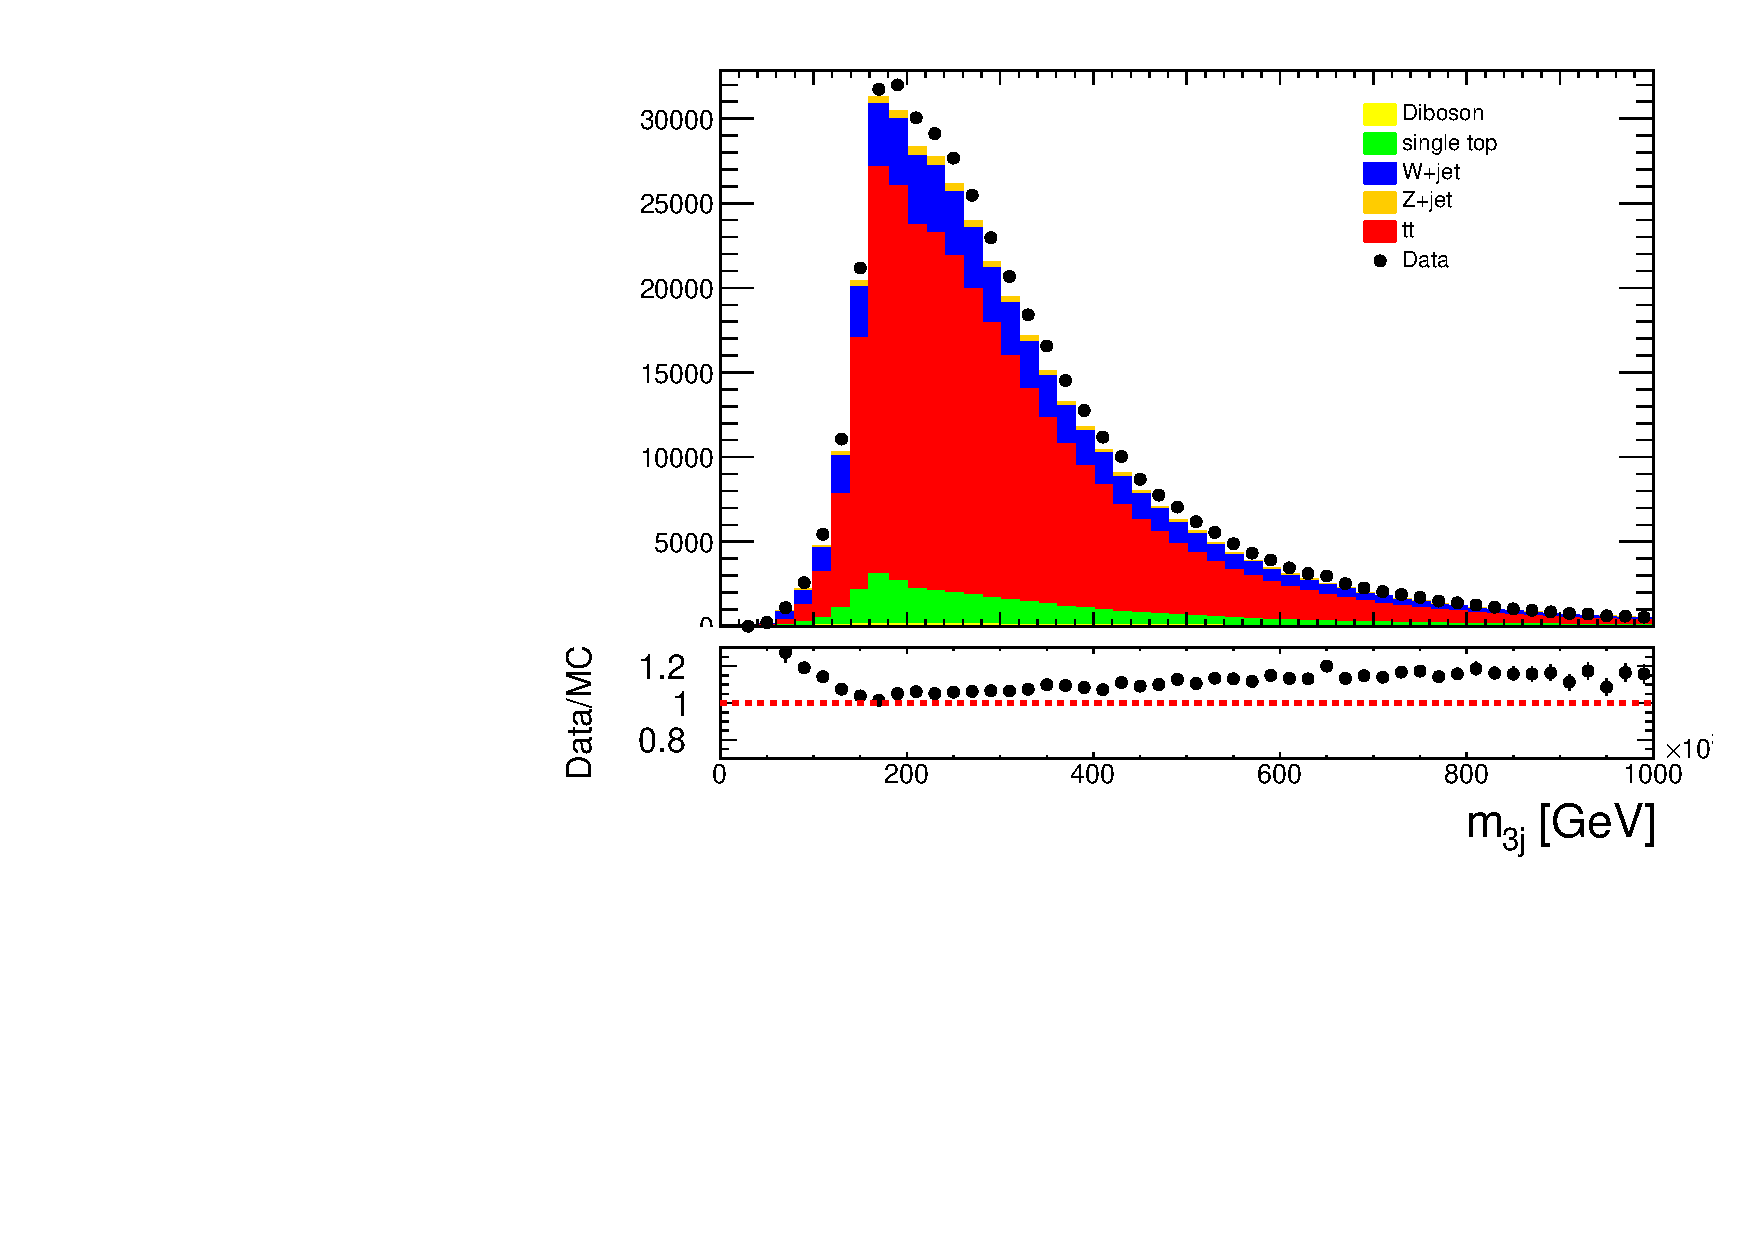
\includegraphics[width=\textwidth]{Figure/h_mc_invM3jet_stacked.pdf}
        \caption{Invariant mass of the three highest-\(p_T\) jets}
        \label{fig:plot_high_c}
    \end{subfigure}
    \hfill
    \begin{subfigure}[b]{0.48\textwidth}
        \centering
        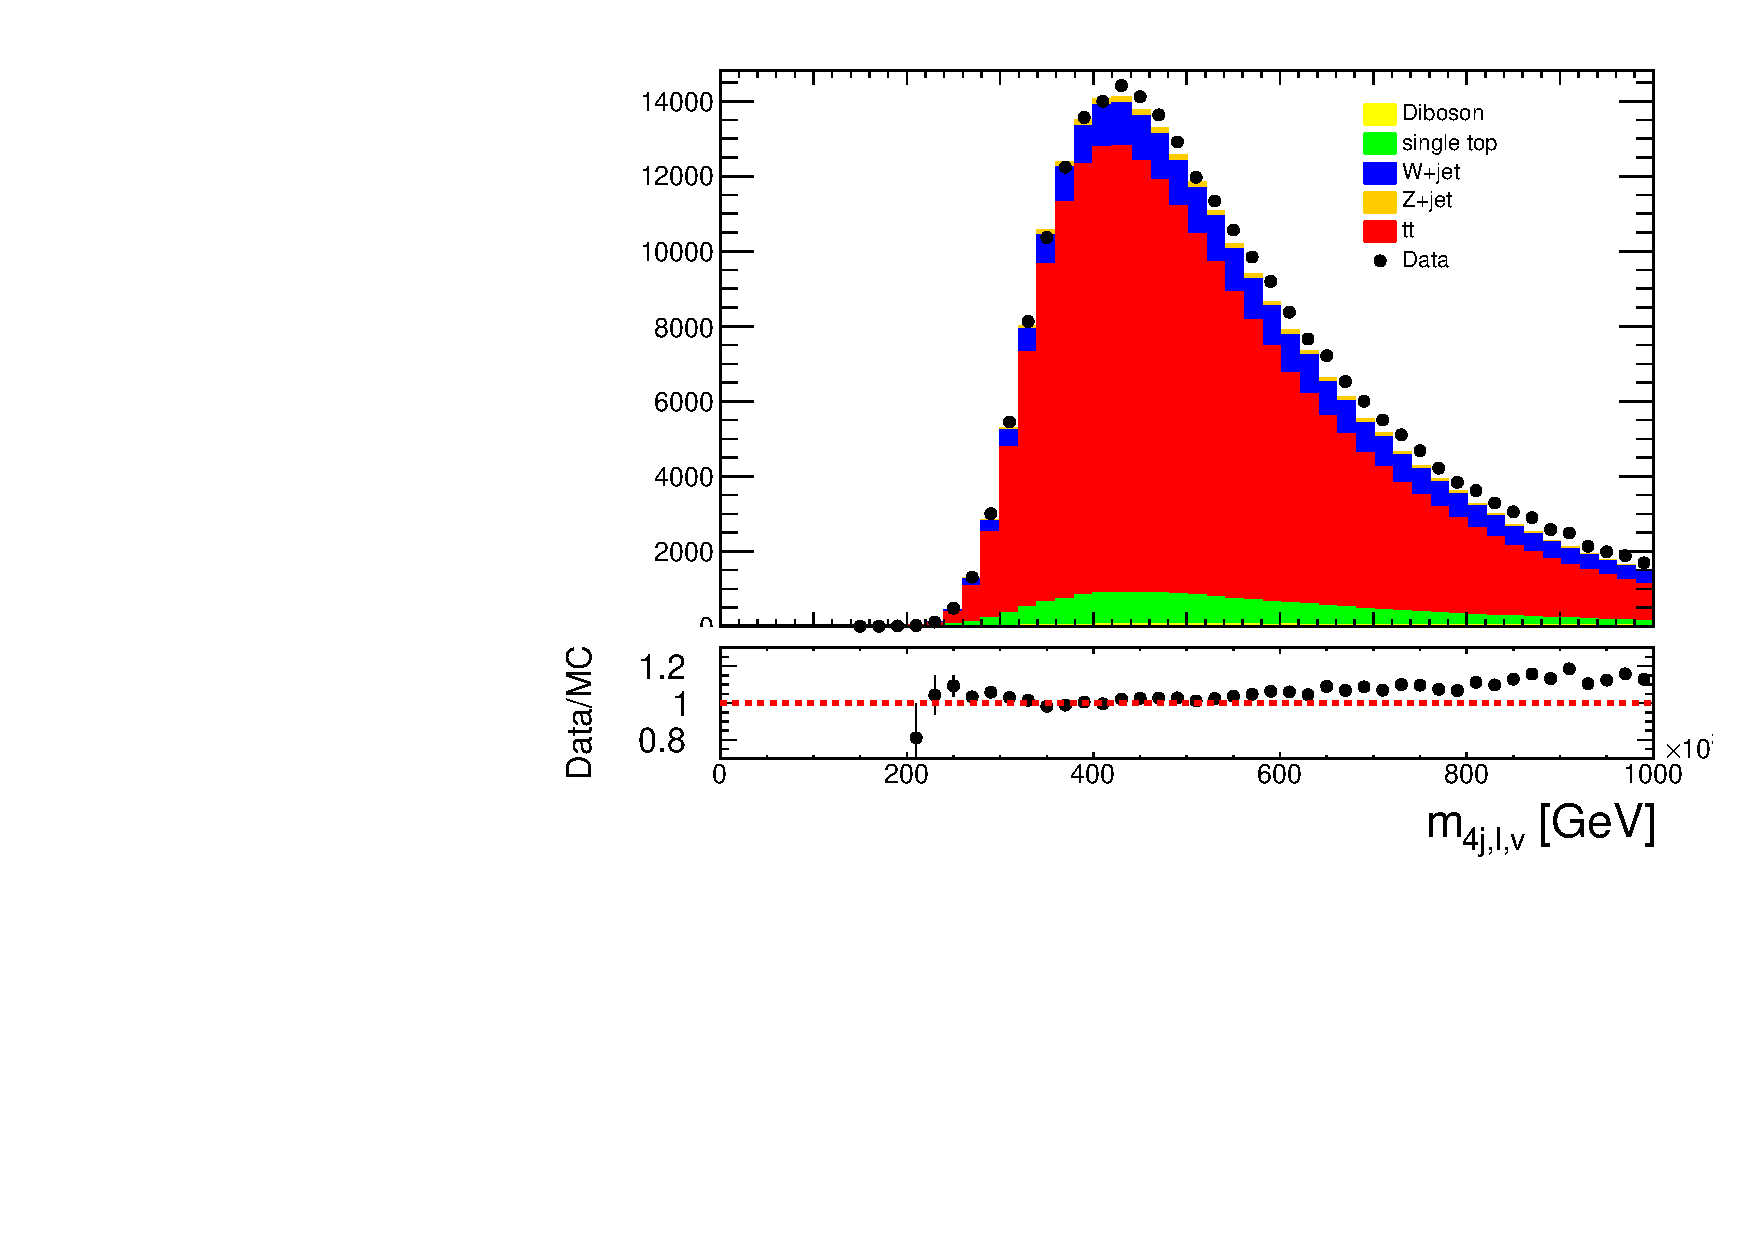
\includegraphics[width=\textwidth]{Figure/h_four_jet_lep_neutrino_inv_mass.pdf}
        \caption{Invariant mass of the four highest-\(p_T\) jets, neutrino and lepton}
        \label{fig:plot_high_d}
    \end{subfigure}

    \caption{Example distributions shown in a stacked plot comparing simulation and data. (a) and (b) reveal some disagreement in the lepton and jet \(p_T\) distributions, In contrast, (c) and (d), which represent higher-level observables, demonstrate good agreement between data and simulation.}
    \label{fig:plot_stack}
\end{figure}


    \section{Statistical analysis}
    The final step is to to evaluate how well the data agree with the Standard Model background. To quantify this agreement, calculating \(\chi^2\) tests if data agrees with the background-only hypothesis. A large \(\chi^2\) value signals possible new physics and helps set exclusion limits on models. The chi-square \(\chi^2\) is defined as

    \begin{equation}
         \chi^2 = \sum_i \frac{(O_i - E_i)^2}{\sigma_i^2}
    \label{eq:chi_square}
    \end{equation}

    where \(O_i\) is the observed number of events in bin \(i\), \(E_i\) is the expected number of events from the SM background in the same bin, and \(\sigma_i\) is the total uncertainty associated with the expected value. However, the \(\chi^2\) alone does not indicate whether the difference is from by random chance. The background-only hypothesis is accepted or rejected based on the p-value defined as:
    \[
    p = P\left(\chi^2_{\text{dof}} \geq \chi^2_{\text{data}}\right)
    \]

    where the degrees of freedom (dof) is defined as
    \[
    \text{dof} = \text{number of bins} - \text{number of fitted parameters} - 1.
    \]
   \\
    Finally, the data can be used for a statistical analysis. Table~\ref{tab:chi2_comparison} shows the results before and after including systematic uncertainties. A flat 14\% uncertainty was added from a 4\% uncertainty in the luminosity and about 10\% from other sources like $b$-tagging and lepton identification.
    \\

\begin{table}[H]
    \centering
    \begin{tabular}{lcc}
        \hline
        \textbf{Statistic} & \textbf{Before Uncertainty} & \textbf{After Uncertainty} \\
        \hline
        \(\chi^2\) & 705.232 & 18.9422 \\
        \(p\)-value & \(1.71 \times 10^{-116}\) & 0.99998 \\
        \hline
    \end{tabular}
    \caption{Comparison of \(\chi^2\) and \(p\)-value before and after including uncertainty.}
    \label{tab:chi2_comparison}
\end{table}

Based on the data before including uncertainties, the \(\chi^2\) value is 705.232 with a \(p\)-value of \(1.71 \times 10^{-116}\), which is far below the \(5\sigma\) threshold of \(5.7 \times 10^{-7}\). This indicates a discovery because it matches an extremely significant deviation from the background-only hypothesis. However, after including uncertainties, the \(p\)-value increases to 0.99998 showing no significant evidence of the \(Z'\) signal.
This results are calculated using the invariant mass of the four highest-$p_{\mathrm{T}}$ jets, the neutrino, and the leptons.




\section{Theoretical Predictions and Exclusion Limits}

Building on this result, we now turn to the theoretical interpretation and constraints derived from the data. Figure \ref{fig:cl} displays the experimental limits on the production of the \(Z'\)-boson as a function of its mass.
\\

The black curve shows the observed 95\% confidence level limit and represents the maximum signal allowed by the data for each mass. The blue curve shows the predicted signal from a \(Z'\)-boson at each mass. If the blue curve is above the black curve, the predicted signal is larger than what the experiment allows. This means those masses are excluded at the 95\% confidence level. No excess was seen up to about 2~\mathrm{TeV}, so \(Z'\)-bosons below this mass are excluded. For higher masses, the predicted signal is too small to test with the current data, and those masses are still possible. This comparison shows which masses are allowed or ruled out by the experiment.





\begin{figure}[H]
    \centering
    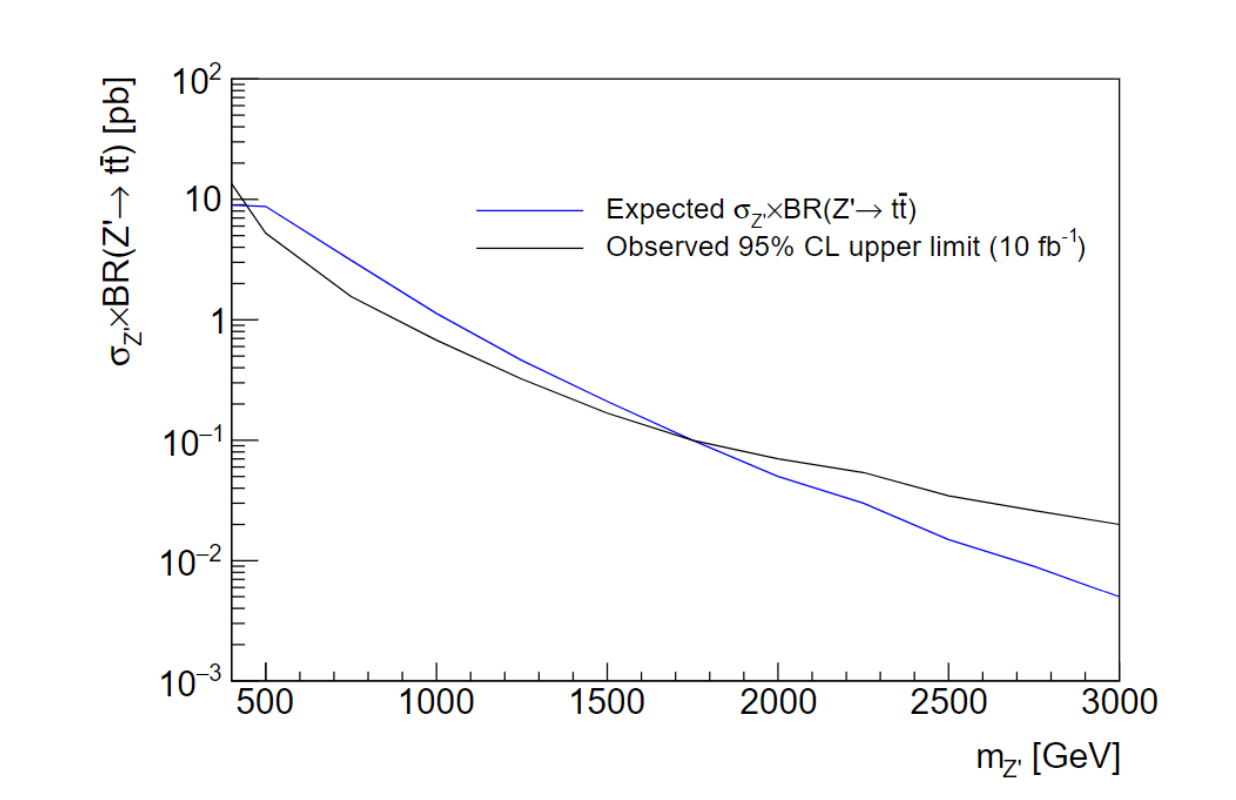
\includegraphics[width=0.6\textwidth]{Figure/CL.png}
    
    \caption{Theoretical limits and 95\% confidence level exclusion limits on the production cross section for various \(Z'\)-boson masses. The x-axis shows the possible mass of the \(Z'\)-boson, while the y-axis shows the production cross section multiplied by the branching ratio for decay into top quarks}

    \label{fig:cl}
\end{figure}













